\section{Análisis de la centralidad de los actores de la red}

Para realizar este análisis se han obtenido los valores de grado, intermediación, cercanía y vector propio de todos los nodos de la red. Se ha realizado sobre la componente gigante para evitar que en otras componentes conexas pequeñas obtengamos valores altos de estas medidas.

Una vez obtenidos estos valores, se ha obtenido la siguiente tabla con los actores más relevantes:


% Please add the following required packages to your document preamble:
% \usepackage{graphicx}
\begin{table}[H]
\centering
\resizebox{\textwidth}{!}{%
\begin{tabular}{|l|l|l|l|}
\hline
\multicolumn{1}{|c|}{\textbf{Centralidad de Grado}} & \multicolumn{1}{c|}{\textbf{Intermediación}}                     & \multicolumn{1}{c|}{\textbf{Cercanía}}                      & \multicolumn{1}{c|}{\textbf{Vector propio}} \\ \hline
Universidad Granada: 2079                           & \textit{Universidad Granada: 1143476,6297}                     & \textit{MIGUEL ÁNGEL: 1}                                 & \textit{Universidad Granada: 1}             \\ \hline
OSL - UGR: 1011                                     & \textit{Residencia Lindaraja Granada: 203280,7911} & \textit{Universidad Granada: 0,6031}                        & \textit{OSL - UGR: 0,7860}                  \\ \hline
UGR emprendedora: 983                               & \textit{OSL - UGR: 171006,8065}                                  & \textit{Residencia Lindaraja Granada: 0,5557} & \textit{UGR emprendedora: 0,7106}           \\ \hline
Delegación ETSIIT: 799                              & \textit{UGR emprendedora: 163371,6347}                           & \textit{UGR Lan Party: 0.5434}                              & \textit{Pilar Aranda UGR: 0,6785}           \\ \hline
Pilar Aranda UGR: 789                               & \textit{UGR Lan Party: 144602,463}                               & \textit{UGR emprendedora: 0,5204}                           & \textit{Delegación ETSIIT: 0,6538}          \\ \hline
\end{tabular}%
}
\caption{Tabla con los actores más relevantes de la red de seguidores de la ETSIIT.}
\end{table}

Voy a empezar por realizar un análisis de las cuentas más relevantes obtenidas sin entrar en detalle de los valores de las medidas, simplemente por ver si tiene sentido que aparezcan estas cuentas.

Como podemos ver, en todos los casos encontramos que la cuenta de la Universidad de Granada es un actor importante para la red en todas las medidas, cosa que tiene sentido ya que al analizar los seguidores de la cuenta de la escuela, todos están relacionados con la Universidad de Granada.

También vemos como la cuenta de UGR Emprendedora es un actor relevante en los seguidores de la ETSIIT. Esto se puede deber a que tanto informática como telecomunicaciones son sectores donde existe un gran interes por el emprendimiento e innovación, además haber tenido durante bastante tiempo a Javier Melero, profesor de la ETSIIT, dentro del equipo de UGR Emprendedora.

Otro de los actores principales acorde a la mayoría de medidas es la Oficina de Software Libre (OSL) de la UGR. Esto tiene sentido ya que se trata de una oficina bastante relacionada con la informática, luego es normal que los seguidores de la escuela de informática conozcan la oficina ya que gran parte de sus actividades se llevan a cabo en la escuela. Además, los directores y directoras de la oficina suelen ser profesores de la ETSIIT, e incluso podemos a los tres últimos directores de la OSL en la red, Pablo García, Juan Julián Merelo y María Isabel García Arenas.

Otros actores que aparecen en un par de medidas son UGR Lan Party, evento organizado por estudiantes del Grado de Ingeniería de Telecomunicación, y la Delegación de estudiantes de la ETSIIT, por lo que podemos intuir que estas asociaciones de estudiantes son importantes en la ETSIIT, además de contar con el propio apoyo de la ETSIIT y la UGR.

También vemos algunas personas concretas, como Pilar Aranda, que al ser la rectora de la UGR cuenta con una alta centralidad de grado, o un caso un poco más raro, con el que vemos a Miguel Ángel con un valor de cercanía de 1. Esto lo vamos a comentar ahora al analizar los valores concretos obtenidos.

Con respecto a los valores concretos obtenidos, voy a comenzar por la centralidad de grado. Podemos ver como claramente el actor con más conexiones es la propia Universidad de Granada, con un valor de grado de 2079 (al ser una red dirigida puede tener más enlaces que nodos en el grafo), más del doble que el segundo actor, la Oficina de Software Libre. Esto se debe a que es normal que quien tenga una conexión con la ETSIIT, también la tiene la UGR ya que forma parte de esta, por lo que es normal que los seguidores de la ETSIIT sigan o sean seguidos por la UGR. Podemos ver que tras esta cuenta encontramos otras cuentas de interés para la comunidad de la ETSIIT, como la Oficina de Software Libre, UGR Emprendedora, la Delegación de estudiantes de la ETSIIT o la cuenta de la rectora de la UGR. Vemos como la diferencia de grado en los últimos actores ya no estan alta, y es que el resto de actores con menos grado no se distinguen tanto, al ser una red con muchas conexiones.

Para la intermediación, la sumatoria del número de caminos mínimos donde se encuentra presente el nodo, vemos como la cuenta de la Universidad de Granada tiene un valor muy alto, casi seis veces mayor que el siguiente. Esto de nuevo se debe a que la cuenta de la UGR, al ser el nodo con mayor grado, y además interconectar cuentas de todo tipo (profesorado, investigadores, estudiantes, empresas, otras cuentas de la UGR, etc), se trata de un nodo muy impotante que actua como hub en la red. También podemos encontrar la cuenta de la Residencia Universitaria Lindarajo Granada en el segundo puesto, y es que como podemos ver en la representación de la red, esta cuenta hace de puente con otra zona más aislada de la red, por lo que gran parte de los caminos mínimos pasan por esa zona, y es considerada importante a nivel de intermediación. A partir de este punto, el resto de actores bajan poco a poco en nivel de intermediación, sin diferencias tan notables, y nos encontramos con cuentas que ocurre como el caso de la UGR, cuentas que interconectan muchas cuentas en la red.

En el caso de la cercanía, tener nodos importantes cerca, vemos un caso extraño, Miguel Angel cuenta con una cercanía de 1, sin embargo, si con Gephi lo localizamos en la red veremos que se trata de un nodo perdido que solo cuenta con tres enlaces:

\begin{figure}[H]
  \centering
  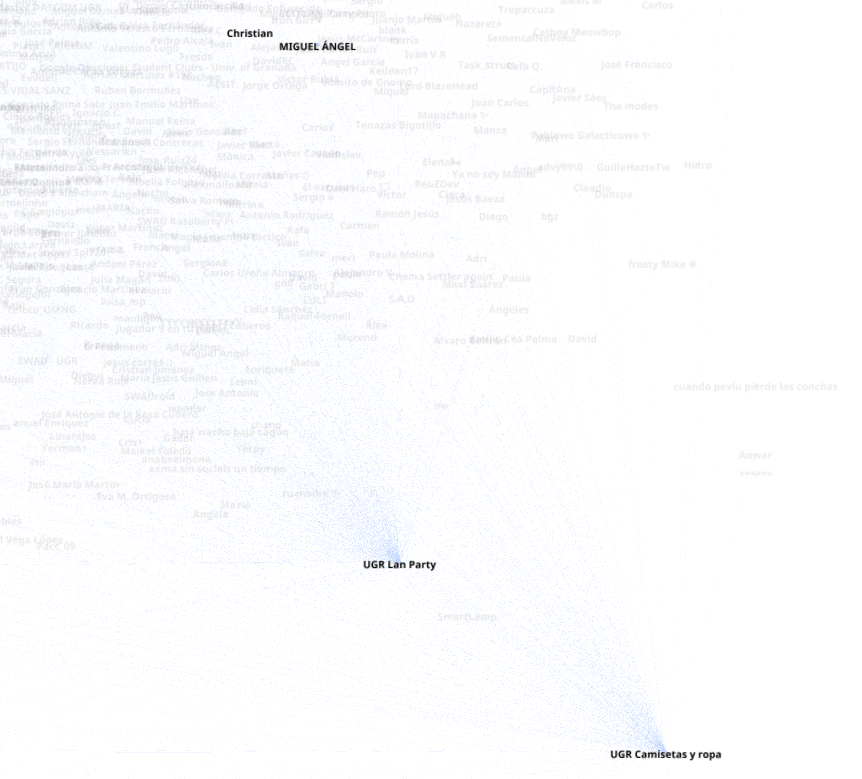
\includegraphics[scale = 0.6]{miguel_angel.png}
  \caption{Nodo de Miguel Ángel seleccionado en la red de seguidores de la ETSIIT.}
  \label{fig:miguel_angel}
\end{figure}

Podemos ver como este nodo se encuentra conectado con la cuenta de UGR Lan Party, que vemos por varias medidas que es una cuenta con importancia, por lo que al estar conectado con tan pocos nodos, pero ser de tanta importancia, de ahí que obtengamos un valor tan alto. Tras este nodo nos encontramos con los nodos de la UGR, la Residencia Lindarajo Granada, UGR Lan Party y UGR Emprendedora con muy poca diferencia en este valor.

Por último, el valor de vector propio (en la que le damos importancia a las conexiones dependiendo de si el nodo con el que se conecta es importante), la cuenta de la UGR obtiene un 1 y es que al tener tantas conexiones, y estar conectada con prácticamente la totalidad de la red, es considerado el nodo más importante de la red. Vemos que el resto de actores son los mismo que los de centralidad de grado, y es que tiene sentido obtener estos resultados por todo lo comentado anteriormente y sabiendo que este valor toma en cuenta la importancia de los nodos conectados y todas estos nodos están conectadas entre si.

En la sección de gráficos adicionales observaremos la red utilizando estos valores para, de forma visual, ver los principales actores de la red.
